\documentclass[english,12pt]{article}

\usepackage{amsthm}
\usepackage[latin9]{inputenc}
\usepackage{babel}
\usepackage[hmargin=0.9in,vmargin=1.25in]{geometry}
\usepackage{graphicx}
\usepackage{subfigure}
\usepackage[colorlinks=true,citecolor=blue,urlcolor=blue]{hyperref}
\usepackage{amsmath}
\usepackage{amssymb,amsfonts}

\newtheorem{theorem}{Theorem}
\newtheorem{lemma}{Lemma}
\newtheorem{cor}{Corollary}

\newcommand{\Rnot}{\sigma_0}
\newcommand{\Sinf}{x_\infty}
\newcommand{\dom}{{\mathcal D}}
\newcommand{\R}{{\mathbb R}}

\DeclareMathOperator\supp{supp}

\begin{document}
\title{Optimal control of an SIR epidemic through short-term non-pharmaceutical intervention}
\author{
  David I. Ketcheson\thanks{Computer, Electrical, and Mathematical Sciences \& Engineering Division,
King Abdullah University of Science and Technology, 4700 KAUST, Thuwal
23955, Saudi Arabia. (david.ketcheson@kaust.edu.sa)}
}
\maketitle

\abstract{We consider the problem of controlling an epidemic within the SIR
framework by temporarily reducing the rate of contact within a population.
The control takes the form of a multiplicative reduction in the contact rate
of infectious individuals.  The control is allowed to be applied only within
a limited time frame, while the objective is to minimize the number of deaths
in the long-time limit subject to some cost function for the control.  Various
specific cost functions are considered and optimal solutions given for each.
Results are applied to the current COVID-19 epidemic.
}

\section{Problem description and assumptions}
The classical SIR model of Kermack \& Mckendrick \cite{} is
\begin{subequations} \label{SIR}
\begin{align} 
    x'(t) & = -\beta y(t) x(t) \label{eq:x} \\
    y'(t) & = \beta y(t) x(t) - \gamma y(t) \label{eq:y} \\
    (x(t_0),y(t_0)) & \in \dom := \{(x_0,y_0) : x_0 \ge 0, y_0\ge 0, x_0+y_0 \le 1\}.
\end{align}
\end{subequations}
With $z(t)=1-x(t)-y(t)$.  The region $\dom$ is forward-invariant
and a unique solution exists for all time.  While the temporal
dynamics of \eqref{SIR} depend on both $\beta,\gamma$, the set
of trajectories depends only on the basic reproduction number 
$\Rnot = \beta/\gamma$.  Dynamics for two values of $\Rnot$ are
shown in Figure \ref{fig:dynamics}.  The system
is at equilibrium if $y(t)=0$; this equilibrium is stable if and
only if $x(t)\le 1/\Rnot$.  If this condition is not satisfied at
the initial time, then $y(t)$ will increase until it is, and then decrease,
approaching zero asymptotically.  The SIR model assumes that recovery
confers permanent immunity.

\begin{figure}
    \centering
    \subfigure[$\sigma=3$]{\label{sigma3}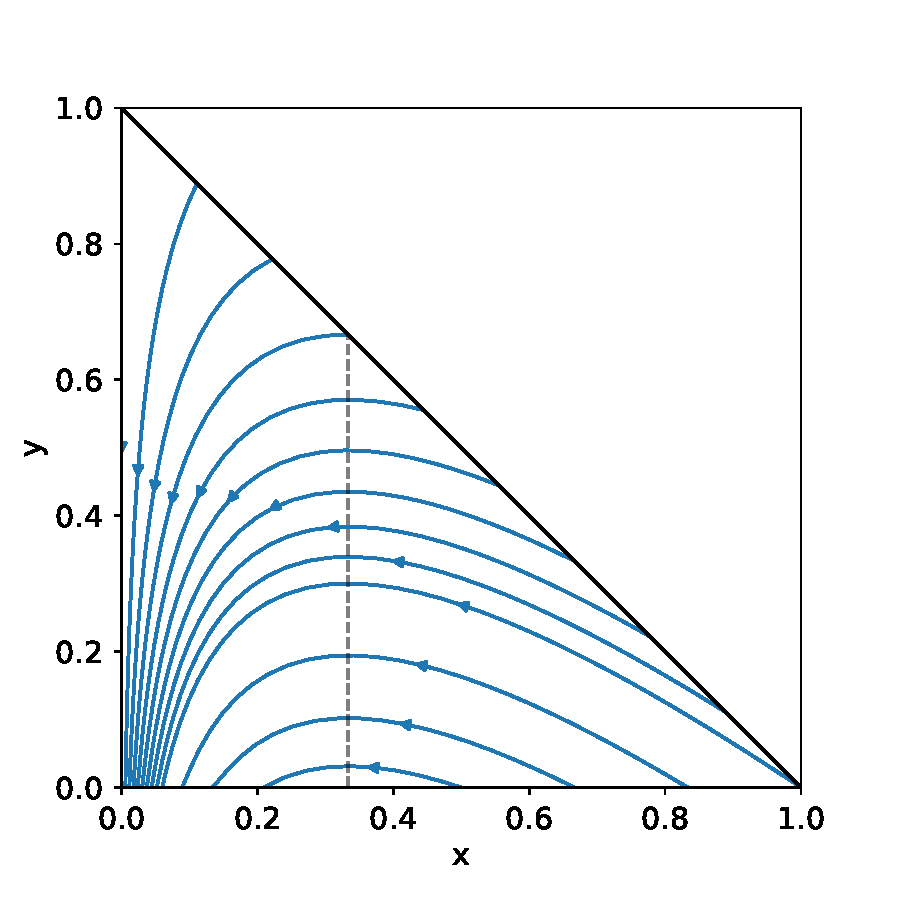
\includegraphics[width=0.49\textwidth]{figures/sigma3.pdf}}
    \subfigure[$\sigma=1.5$]{\label{sigma15}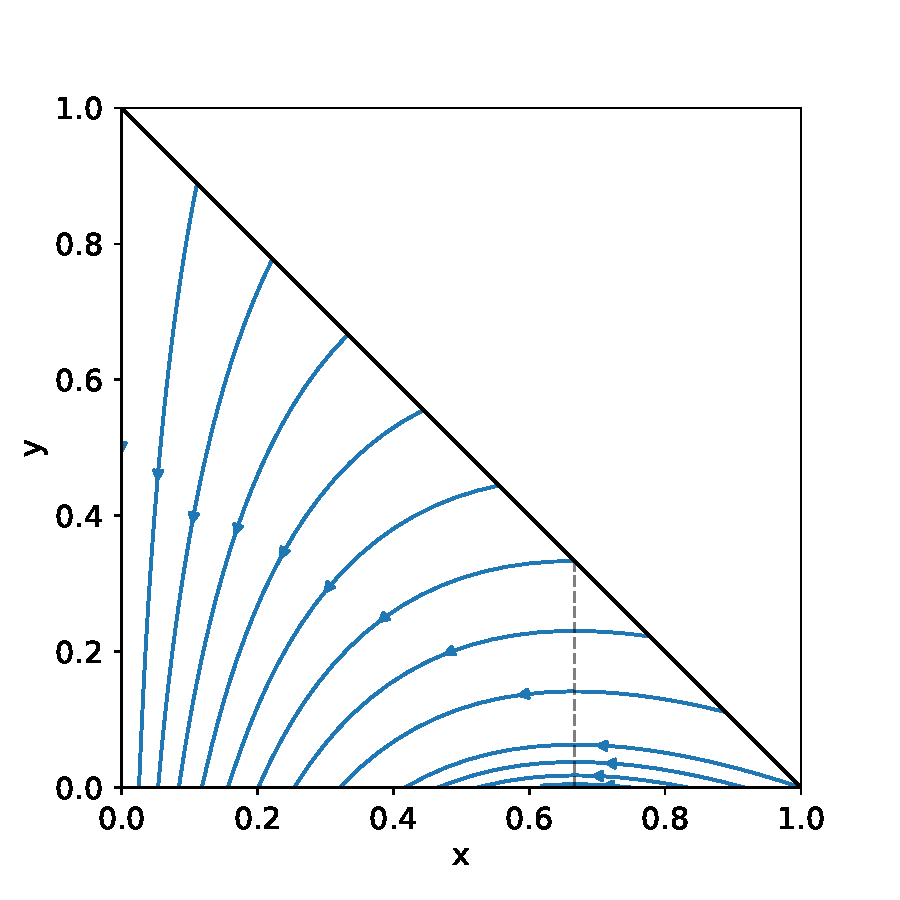
\includegraphics[width=0.49\textwidth]{figures/sigma15.pdf}}
    \caption{Dynamics of SIR model for two values of the basic reproduction number.
            The critical value $x=1/\sigma$ is shown with a dashed line.\label{fig:dynamics}}
\end{figure}

To prevent an epidemic it is necessary to reduce the susceptible
fraction to the level $1/\Rnot$; this is often referred to as {\em herd
immunity}.  For many diseases affecting humans, herd immunity is achieved
through vaccination if a sufficient portion of the population.  If a vaccine
is unavailable, herd immunity can only be achieved through infection and recovery.
In an epidemic the susceptible population will eventually be reduced
to less than the critical value $1/\Rnot$, since this value only governs
when the infected fraction will begin to decrease.  Additional individuals
will be infected after this point; this is referred to as {\em epidemiological
overshoot}.

We model a non-pharmaceutical intervention (NPI) control via a time-dependent
parameter $q(t)\in[0,1]$ with the qSIR system
\begin{subequations} \label{SIRq}
\begin{align}
    x'(t) & = -(1-q(t))\beta y x \\
    y'(t) & = (1-q(t))\beta y x - \gamma y
\end{align}
\end{subequations}
The effect of $q$ is to effectively reduce the reproduction number which is now
given by $\sigma(t) = (1-q(t))\Rnot$.  This can account for both
population-wide interventions and interventions specific to identified infectious
(or possibly infectious) individuals.  

Most epidemics do not result in substantial permanent changes in the contact rate of
a population.  We therefore assume that intervention can only be applied over a limited
time, up to $t_*$.  Thus 
\begin{align} \label{q-shortterm}
    q(t)=0 \text{ for } t>t_*.
\end{align}

Our objective is to minimize $z_\infty := \lim_{t \to \infty} z(t)$, or equivalently
(since $y_\infty=0$)
to maximize $\Sinf := \lim_{t \to \infty} x(t)$.  This has the effect of minimizing
the number of eventual deaths, which would be proportional to $z_\infty$.

We state the control problem as follows:
\begin{align}
\text{Choose } q(t) \text{ to minimize } f(q) \text{ subject to \eqref{SIRq}, \eqref{q-shortterm}, and} \\
x(\infty;q) = 1/\sigma.
\end{align}


\section{Preliminaries}
We define the solution operator $\phi_t(\beta,\gamma): \dom \to \dom$ as the map
that takes an initial condition $(x_0,y_0)$ to the solution $(x(t),y(t))$
via the solution of \eqref{SIR}.  We further define for $u\in\dom$
$$
    x_\infty(u,\sigma) = \lim_{t\to\infty} \phi_t(\sigma,1)u.
$$
Observe that each trajectory in Figure \ref{fig:dynamics} is a contour of $x_\infty$.
Our objective then is to minimize $x_\infty((x(t_*),y(t_*)),\Rnot)$.
By applying the control we can move the solution to a different contour of
$x_\infty(\cdot,\sigma)$.  First we show that applying any control $q>0$ over
any length of time leads to a decrease in $x_\infty$.

\begin{lemma}
Let $\Rnot>0$ and $u\in\dom$ be given and define $X_\infty = x_\infty(u,\Rnot)$.
Then for any $0<\sigma<\Rnot$ and any $t>0$ we have
$$
    x_\infty(\phi_t(\sigma,1)u,\Rnot) > X_\infty.
$$
\end{lemma}
\begin{proof}
    Dividing \eqref{eq:y} by \eqref{eq:x} gives
    $$
        \frac{dy}{dx} = -1 + \frac{1}{\sigma s}.
    $$
    Thus reducing $\sigma$ has the effect of increasing $dy/dx$.
    Since all trajectories flow to the left ($x$ is a decreasing function of $t$),
    this means that $\phi_t(\sigma,1)u$ lies below $\phi_t(\Rnot,1)u$ for all $t>0$.
\end{proof}

\begin{cor} \label{cor:diff-control}
Let two control functions $q(t), \hat{q}(t)$ be given with $\hat{q(t)}<q(t)$.
Then $x_\infty(q)>x_\infty(\hat{q})$.
\end{cor}

In the classic SIR model, the asymptotic susceptible fraction $\Sinf$ is
given as a function of the initial state and of $\Rnot$ by the unique solution 
in the interval $(0,1/\Rnot)$ of the
following equation \cite[Eqn. (5.4)]{hethcote1989three}:
\begin{align} \label{s-infty}
    1 - z_0 - \Sinf + \frac{1}{\Rnot} \log\left(\frac{\Sinf}{x_0}\right) = 0.
\end{align}

\begin{theorem}
Let $y_0>0$ and
let $\Sinf(q) = \lim_{t\to\infty} x(t;q)$ where $x(t;q)$ denotes the solution of
\eqref{SIRq} subject to \eqref{q-shortterm}.  Then $\Sinf\le 1/\sigma$.
\end{theorem}
\begin{proof}
Due to condition \eqref{q-shortterm}, as $t \to \infty$ the solution of \eqref{SIRq}
must tend to a stable equilibrium point of \eqref{SIR}.  But the stable equilibrium
points of \eqref{SIR} satisfy $x \le 1/\sigma$.
\end{proof}

It is straightforward to show that $x(t)$ satisfies (see e.g. \cite{harko2014exact,pakes2015lambert})
$$
    x(t) = x_0 e^{\sigma(z_0-z(t))}.
$$
Since $z=1-x-y$ we find that
$$
   \mu(x_0,y_0) := x_0 e^{-\sigma(x_0+y_0)} =  x(t) e^{-\sigma(x(t)+y(t))} 
$$
In other words, $\mu$ is constant in time, and the trajectories
in Figure \ref{fig:dynamics} are contours of $\mu$.
Since also $y_\infty=0$, we have
$$
    x_\infty = x_0 e^{\sigma(x_\infty-x_0-y_0)} = \mu(x_0,y_0) e^{\sigma x_\infty}.
$$
Setting $w=-x_\infty \sigma$ we have
$$
    we^w = -x_0 \sigma e^{-\sigma(x_0+y_0)} = -\mu \sigma.
$$
Thus $w = W_0(-\mu\sigma)$ where $W_0$ is the principal branch of Lambert's $W$-function \cite{pakes2015lambert},
and
$$
    x_\infty = -\frac{1}{\sigma}W_0(-\mu \sigma).
$$



\section{Optimal controls}
No trajectory starting from $y_0>0$ reaches $y(t)=0$ in finite time, regardless of the
value of $\sigma$.  Hence it is impossible to reach the optimal equilibrium state
$(1/\sigma_0,0)$ with a finite-time control.  Therefore we look for $\epsilon$-optimal
solutions that tend to an equilibrium $(x_\infty,0)$ with $x_\infty > 1/\sigma_0 - \epsilon$.

\subsection{Minimization of the maximum control}
\begin{align} \label{eq:minmax}
\text{ Minimize } \max_t(q(t)) \text{ subject to } \eqref{SIRq} \text{ and } x_\infty > \frac{1}{\sigma} - \epsilon.
\end{align}
Solution is to take $q(t)=q_*$ for all $t<t_*$, where $q_*$ is chosen so that $x_\infty(u_0,\sigma(q_*))=1/\sigma_0$.


\subsection{Minimization of the length of control}
\begin{align} \label{eq:minsupp}
\text{ Minimize } \supp(q(t)) \text{ subject to } \eqref{SIRq} \text{ and } x_\infty > \frac{1}{\sigma} - \epsilon.
\end{align}

\begin{lemma} \label{lem:maxq}
    {\bf (Bang-bang control)}
    If there exists an optimal control for \eqref{eq:minsupp}, then there exists
    an optimal control with the property that for each $t$, either $q(t)=0$ or $q(t)=1$.
\end{lemma}
\begin{proof}
    Let an optimal control be given such that for some subset of $(t_0,t_*)$, $q(t)\in(0,1)$.
    Then by Corollary \ref{cor:diff-control}, the control where for all such $t$ $q(t)=1$
    is also optimal.  (can make this stronger)
\end{proof}

Taking $q(t)=1$, the system \eqref{SIRq} becomes simply
\begin{subequations}
\begin{align}
    x'(t) & = 0 \\
    y'(t) & = - \gamma y
\end{align}
\end{subequations}
with solution
\begin{subequations} \label{qone}
\begin{align}
    x(t) & = x(t_0) \\
    y(t) & = e^{-\gamma t} y(t_0).
\end{align}
\end{subequations}

\begin{theorem}
An optimal control for \eqref{eq:minsupp} is given by
\begin{align}
    q(t) & = \begin{cases}  
        0 & t<t_{\max} \\
        1 & t_{\max}\le t \le t_* \\
        0 & t>t_*,
    \end{cases}
\end{align}
where $t_{\max}$ is the time at which $x(t)=1/\sigma$ and $t_*$ is the time
at which $x_\infty=1/\sigma-\epsilon$ (need to work these out).
\end{theorem}
\begin{proof}
    Due to Lemma \ref{lem:maxq}, we know there is an optimally-controlled
    trajectory that consists piecewise of the dynamics given by \eqref{SIR}
    and those given by \eqref{qone}.  In other words, an optimal control consists
    of a set of intervals over which $q(t)=1$.  To minimize the support of $q(t)$
    it is necessary and sufficient to maximize the average rate of improvement
    in $x_\infty$ over these intervals.  This rate is
    \begin{align*}
        \left. \frac{dx_\infty}{dt}\right|_{x=x_0} = \left. \frac{dx_\infty}{dy}\right|_{x=x_0} \frac{dy}{dt} \\
            & = -\gamma y \left. \frac{dx_\infty}{dy}\right|_{x=x_0}
    \end{align*}
    Using the identity $W'(z) = 1/(z+e^{W(z)})$ we have
    \begin{align*}
        \left. \frac{dx_\infty}{dy}\right|_{x=x_0} = \frac{-\mu \sigma}{e^{-\sigma x_\infty}-\mu\sigma},
    \end{align*}
    which is constant along SIR trajectories (since both $\mu$ and $x_\infty$ are constant).
    Thus the effectiveness of the control is maximized by applying it at the maximum
    value of $y$ for each $x_\infty$, and each contour of $x_\infty$ has its maximum
    at $x=1/\sigma$.
\end{proof}
Add some plots of optimal and non-optimal control trajectories.

\subsection{Minimization of the square integral of the control}

\bibliographystyle{plain}
\bibliography{refs}

\end{document}
